\documentclass[a4paper,10pt]{article} 
\usepackage[utf8]{inputenc}
\usepackage[a4paper]{geometry}
\usepackage[magyar]{babel}
\usepackage{amsmath}
\usepackage{amssymb}
\usepackage{wrapfig}
\usepackage{pgf, tikz}
\frenchspacing 
\pagestyle{empty}
\newcommand{\ki}[2]{\hfill {\it #1 (#2)}\medskip}
\newcommand{\vonal}{\hbox to \hsize{\hskip2truecm\hrulefill\hskip2truecm}}
\newcommand{\degre}{\ensuremath{^\circ}}
\newcommand{\tg}{\mathop{\mathrm{tg}}\nolimits}
\newcommand{\ctg}{\mathop{\mathrm{ctg}}\nolimits}
\newcommand{\arc}{\mathop{\mathrm{arc}}\nolimits}
\begin{document}
\begin{center} \Large {\em 24. Nemzetközi Magyar Matematika Verseny} \end{center}
\begin{center} \large{\em Szabadka, 2015. április 8-12.} \end{center}
\smallskip
\begin{center} \large{\bf 9. osztály} \end{center}
\bigskip 

{\bf 1. feladat: } Egy
$20 \times 20$-as négyzetháló négyzeteibe a bal
felső mezőből indulva soronként  
sorra beírjuk az
$1, 2, 3,\ldots , 400$
pozitív egész számokat.
Ezután a
táblázat négyzeteiből az ábrán látható kereszt
alakú síkidommal mindig ötöt letakarunk az összes
lehetséges módon.\\
\centerline{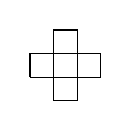
\begin{tikzpicture}[x=0.3cm,y=0.3cm]
\clip (-0.1,-0.1) rectangle (3.1,3.1);
\draw (1,0)--(2,0)--(2,3)--(1,3)--(1,0);
\draw (0,1)--(3,1)--(3,2)--(0,2)--(0,1);
\end{tikzpicture}}\\
Hányszor lesz a letakart öt szám
összege négyzetszám? Milyen szám áll ezekben az
esetekben a kereszt közepén?

\ki{Nemecskó István}{Budapest, Magyarország}\medskip

{\bf Megoldás: } Ha a kereszt középső mezőjében $k$ áll, akkor az öt mező összege $5k$. Ha ez négyzetszám, akkor $5\mid k$ teljesül. A középső mező viszont nem lehet a tábla szélén, ezért: $20<k<380$, valamint $k\ne 20i$, ha $i=1,2,\ldots,20$,  és  $k\ne 20j+1$, ha $j=0, 1, \ldots,19$. Mivel $5k$ négyzetszám, így $k=5\cdot l^2$ alakú, ahol $l$ természetes szám. Az előző feltételek miatt adódik, hogy $4<l^2<76$, ebből pedig $2<l<9$.
 
 $l=3$ esetén $k=5\cdot 3^2=45$, ami teljesíti a feltételt.
 
 $l=4$ esetén $k=5\cdot 4^2=80$, ami nem teljesíti a feltételt.
 
 $l=5$ esetén $k=5\cdot 5^2=125$, ami teljesíti a feltételt.
 
 $l=6$ esetén $k=5\cdot 6^2=180$, ami nem teljesíti a feltételt.
 
 $l=7$ esetén $k=5\cdot 7^2=245$, ami teljesíti a feltételt.
 
 $l=8$ esetén $k=5\cdot 8^2=320$, ami nem teljesíti a feltételt.
 
A megfelelő értékek tehát $l=3$, $l=5$ és $l=7$, s így a letakart keresztek középső mezői, rendre, 45, 125 és 245 lehetnek.

\vonal

{\bf 2. feladat: } Egy háromjegyű számot osztva a számjegyeinek összegével $37$-et kapunk. Ha e
háromjegyű számhoz hozzáadunk $297$-et, a megfordított (felcserélt sorrendben
felírt) számjegyek\-ből álló számot kapjuk. Mely háromjegyű számok esetében
lehetséges ez?

\ki{Kovács Béla}{Szatmárnémeti, Erdély}\medskip

{\bf Megoldás: } Legyen a háromjegyű szám $100a+10b+c$. Az első feltétel alapján adódik $100a+10b+c=37(a+b+c)$, innen pedig $63a=27b+36c$. Elosztva 9-cel a kapott egyenletet, kapjuk a $7a=3b+4c$ összefüggést. A második feltétel alapján adódik a $100a+10b+c+297=100c+10b+a$ egyenlet, innen pedig $99a+297=99c$, amely 99-cel osztva adja az $a+3=c$ összefüggést. Az első egyenlőségbe helyettesítve kapjuk, hogy $7a=3b+4(a+3)$, ahonnan $3a=3b+12$, amely 3-mal osztva adja az $a=b+4$  egyenlőséget. Tehát: $a=b+4$ és $c=b+7$. Mivel $a, b, c$  számjegyek, ezért $b$ lehetséges értékei: $0$, $1$ vagy $2$.
 
Ha $b=0$, akkor $a=4$ és $c=7$, a keresett háromjegyű szám pedig a 407.

Ha $b=1$, akkor $a=5$ és $c=8$, a keresett háromjegyű szám pedig az 518.

Ha $b=2$, akkor $a=6$ és $c=9$, a keresett háromjegyű szám pedig a 629.

\noindent
A keresett háromjegyű számok tehát: 407, 518 és 629.
$407:11=37$ és $704-407=297$, 
$518:14=37$ és $815-518=297$,
$629:17=37$ és $926-629=297$.

\vonal

{\bf 3. feladat: } Hány megoldása van a prímszámok halmazában a
$p^2 + q^2 + r^2 + s^2 = pqrs + 4$
egyenletnek?

\ki{Mészáros József}{Galánta, Felvidék}\medskip

{\bf Megoldás: } Mind a négy prímszám nem lehet páratlan. Tegyük fel, hogy $s=2$. Ekkor
$$p^2+q^2+r^2=2pqr.$$
A megmaradt prímszámok sem lehetnek mind páratlanok, mert akkor a bal oldal páratlan volna a jobb oldal pedig páros. Legyen $r=2$. Ekkor \\
\centerline{$p^2+q^2+4=4pq$,   illetve  $p^2+q^2=4(pq-1)$.\\}
A bal oldali kifejezés miatt $p$ és $q$ paritása megegyező kell, hogy legyen. Ha mindkettő páratlan volna, akkor $p^2=4k+1$ és $q^2=4l+1$ alakú, ahol $k$ és $l$ valamilyen pozitív egész számok. Ekkor viszont a $p^2+q^2=4(pq-1)$ egyenlet bal oldala $4m+2$ alakú, ahol $m$ pozitív egész szám, a jobb oldala pedig 4 többszöröse. Következésképpen csak a  $p=q=2$ eset lehetséges. Ekkor viszont $4+4=4\cdot 3$, ami ellentmondás, tehát az adott egyenletnek nincs a feladat feltételeit kielégítő megoldása.

\vonal

{\bf 4. feladat: } Egy $ABC$
háromszögben
$A \sphericalangle = 60^\circ$. 
Legyenek rendre az $M$ és $N$
pontok az $AB$ és $AC$
oldalak olyan pontjai, melyekre
$AM = CN$. 
Az $MN$ szakasz felezőpontja legyen $F_1$, míg az $AC$
oldal felezőpontja $F_2$. Bizonyítsd be, hogy
$$F_1F_2 = \frac{1}{2}\cdot AM. $$

\ki{Bíró Béla}{Sepsiszentgyörgy, Erdély}\medskip

{\bf 1. megoldás: } Tekintsük az $A$ csúcsnak az $F_1$ pontra vonatkozó $A_1$ szimmetrikus képét. (lásd az ábrát) A feltevést is figyelembe véve, az $AMA_1N$ négyszög paralelogramma.
Így $AM=A_1N$ és $AM \parallel A_1N$. Emiatt $A_1N=NC$ és $BAC\sphericalangle=A_1NC\sphericalangle=60^\circ$, ahonnan következik, hogy az $A_1NC_{\Delta}$ szabályos. Következésképpen $A_1C=NC=AM$.
Végezetül: $F_1F_2$ középvonal az $AA_1C$ háromszögben, s ebből az következik, hogy 
$F_1F_2=\dfrac{1}{2}\cdot A_1C=\dfrac{1}{2}\cdot AM$, amit igazolni kellett.

\begin{center}
\definecolor{uuuuuu}{rgb}{0.266666666667,0.266666666667,0.266666666667}
\begin{tikzpicture}[line cap=round,line join=round,x=1.0cm,y=1.0cm]
%\clip(-1.96,-1.42) rectangle (6.74,4.92);
\draw (-1.23839666658,3.02008191467)-- (5.25614150823,0.487407958784);
\draw (-1.25211147532,-0.0600351251611)-- (6.33792341242,-0.143598121707);
\draw (-1.23282032303,4.2724355653)-- (-1.25211147532,-0.0600351251611);
\draw (-1.23282032303,4.2724355653)-- (6.33792341242,-0.143598121707);
\draw (2.5525515447,2.0644187218)-- (2.00887242082,1.75374493673);
\draw [dash pattern=on 2pt off 2pt] (6.33792341242,-0.143598121707)-- (5.25056516467,-0.764945691846);
\draw [dash pattern=on 2pt off 2pt] (5.25056516467,-0.764945691846)-- (5.25614150823,0.487407958784);
\draw [dash pattern=on 2pt off 2pt] (5.25056516467,-0.764945691846)-- (-1.23282032303,4.2724355653);
\begin{scriptsize}
\draw [fill=uuuuuu] (-1.23282032303,4.2724355653) circle (1.5pt);
\draw[color=uuuuuu] (-1.1,4.56) node {$A$};
\draw [fill=uuuuuu] (-1.25211147532,-0.0600351251611) circle (1.5pt);
\draw[color=uuuuuu] (-1.12,0.22) node {$B$};
\draw [fill=uuuuuu] (6.33792341242,-0.143598121707) circle (1.5pt);
\draw[color=uuuuuu] (6.48,0.14) node {$C$};
\draw [fill=uuuuuu] (-1.23839666658,3.02008191467) circle (1.5pt);
\draw[color=uuuuuu] (-1.1,3.3) node {$M$};
\draw [fill=uuuuuu] (5.25614150823,0.487407958784) circle (1.5pt);
\draw[color=uuuuuu] (5.4,0.76) node {$N$};
\draw [fill=uuuuuu] (2.00887242082,1.75374493673) circle (1.5pt);
\draw[color=uuuuuu] (1.96,1.54) node {$F_1$};
\draw [fill=uuuuuu] (2.5525515447,2.0644187218) circle (1.5pt);
\draw[color=uuuuuu] (2.74,2.4) node {$F_2$};
\draw [fill=uuuuuu] (5.25056516467,-0.764945691846) circle (1.5pt);
\draw[color=uuuuuu] (5.22,-0.98) node {$A_1$};
\end{scriptsize}
\end{tikzpicture}
\end{center}

{\bf 2. megoldás: } Az általánosság megszorítása nélkül feltehetjük, hogy az $ABC_{\Delta}$ hegyesszögű, és az $AB$ oldala hosszabb az $AC$ oldalnál. A háromszög $AC$ oldalán vegyünk fel egy $D$ pontot úgy, hogy $AM=AD$ legyen. Ekkor az $AMD_{\Delta}$ egyenlő oldalú, ugyanis $AM=AD$, valamint az $A$ csúcsban lévő szög $60^\circ$. Mivel az $F_2$ pont az $AC$ szakasz felezőpontja, és $AD=AM=CN$, így az $F_2$ pont a $DN$ szakasznak is a felezőpontja. Az  $MND_{\Delta}$-ben ezek alapján $F_1F_2$ a háromszög középvonala, vagyis
 $$F_1F_2=\frac{1}{2}\cdot MD.$$
 \begin{center}
 \definecolor{uuuuuu}{rgb}{0.26666666666666666,0.26666666666666666,0.26666666666666666}
\begin{tikzpicture}[line cap=round,line join=round,x=1.0cm,y=1.0cm]
%\clip(-1.9400000000000002,-0.6600000000000037) rectangle (4.739999999999998,4.659999999999998);
\draw (-1.2383966665790722,3.0200819146676308)-- (3.2142370545887697,1.6784559149698046);
\draw (-1.2529109611625027,-0.23958629622001465)-- (4.296018958781277,1.047449834478665);
\draw (-1.2328203230275496,4.272435565298213)-- (-1.2529109611625027,-0.23958629622001465);
\draw (-1.2328203230275496,4.272435565298213)-- (4.296018958781277,1.047449834478665);
\draw (1.5315993178768634,2.6599426998884392)-- (0.9879201940048488,2.3492689148187176);
\draw [dash pattern=on 1pt off 1pt] (-1.2383966665790722,3.0200819146676308)-- (-0.15103841883504285,3.641429484807074);
\begin{scriptsize}
\draw [fill=uuuuuu] (-1.2328203230275496,4.272435565298213) circle (1.5pt);
\draw[color=uuuuuu] (-1.5800000000000003,4.399999999999999) node {$A$};
\draw [fill=uuuuuu] (-1.2529109611625027,-0.23958629622001465) circle (1.5pt);
\draw[color=uuuuuu] (-1.5200000000000002,-0.04000000000000342) node {$B$};
\draw [fill=uuuuuu] (4.296018958781277,1.047449834478665) circle (1.5pt);
\draw[color=uuuuuu] (4.439999999999999,1.3199999999999972) node {$C$};
\draw [fill=uuuuuu] (-1.2383966665790722,3.0200819146676308) circle (1.5pt);
\draw[color=uuuuuu] (-1.6200000000000003,3.079999999999998) node {$M$};
\draw [fill=uuuuuu] (3.2142370545887697,1.6784559149698046) circle (1.5pt);
\draw[color=uuuuuu] (3.359999999999999,1.9599999999999973) node {$N$};
\draw [fill=uuuuuu] (0.9879201940048488,2.3492689148187176) circle (1.5pt);
\draw[color=uuuuuu] (0.9399999999999993,2.1199999999999974) node {$F_1$};
\draw [fill=uuuuuu] (1.5315993178768634,2.6599426998884392) circle (1.5pt);
\draw[color=uuuuuu] (1.7199999999999993,2.999999999999998) node {$F_2$};
\draw [fill=uuuuuu] (-0.15103841883504285,3.641429484807074) circle (1.5pt);
\draw[color=uuuuuu] (-0.020000000000000566,3.919999999999998) node {$D$};
\end{scriptsize}
\end{tikzpicture}
 \end{center}
Figyelembe véve az $AMD_{\Delta}$ egyenlő oldalú voltát megkapjuk a feladat bizonyítandó állítását:
$$F_1F_2=\frac{1}{2}\cdot MD=\frac{1}{2}\cdot AM.$$
\textit{Megjegyzés}: ha a $CN$ szakasz hossza nagyobb a $CF_2$ szakaszétól, a feladat megoldása akkor is hasonlóan alakul a fentiekhez.

\vonal

{\bf 5. feladat: } Keresd meg az összes olyan pozitív egészekből álló
 $(x , y , z)$ 
számhármast,
amelyre érvényes, hogy
$ x \mid (y + 1),\quad 2y \mid (z+2) \quad
\text{~és~}\quad
3z \mid (x + 3)$.

\ki{Kekeňak Szilvia}{Kassa, Felvidék}\medskip

{\bf Megoldás: } Az $ x \mid (y + 1),\quad 2y \mid (z+2) \quad
\text{~és~}\quad
3z \mid (x + 3)$ feltételekből következik, hogy 
$x\le y+1$, $2y\le z+2$ és $3z\le x+3$.
Szorozzuk be az első egyenlőtlenséget 2-vel és alkalmazzuk egymás után az első két egyenlőtlenséget. Ekkor azt kapjuk, hogy 
$2x\le 2y+2\le z+4$, illetve hogy $2x-4\le z$.
Figyelembe véve a $2x-4\le z$ és a $3z\le x+3$ egyenlőtlenségeket adódik, hogy 
$3(2x-4)\le 3z\le x+3$, azaz $3(2x-4)\le x+3$.
Az utóbbi egyenlőtlenség megoldása $x\le 3$. A $3z\mid (x+3)$  feltételből következik, hogy $3\mid (x+3)$, ezért $3\mid x$, így az $x\le 3$ feltételt is figyelembe véve adódik, hogy $x=3$.

Figyelembe véve a $3z\mid (x+3)$ feltételt, azt kapjuk, hogy $3z\mid 6$, vagyis $z\mid 2$.
Mivel $2y\mid (z+2)$ alapján $z$ biztosan páros szám, így $z=2$. 

Visszahelyettesítve a kapott értékeket a $2x\le 2y+2\le z+4$ egyenlőtlenségbe, adódik, hogy $6\le 2y+2 \le 6$, ahonnan $y=2$.

A feladat egyetlen megoldása tehát a $(3,2,2)$ számhármas. 

\vonal

{\bf 6. feladat: }  Az $ABC$
hegyesszögű háromszög magasságpontja $M$. 
Igazold, hogy ha $MC = AB$, akkor az
$ACB\sphericalangle=45^\circ$. 
Igaz-e az állítás tompaszögű háromszögben is?


\ki{Katz Sándor}{Bonyhád, Magyarország}\medskip

{\bf Megoldás: } Az ábrán $\alpha$-val jelölt $ABT$ és $TCM$ szögek egyenlők, mert merőleges szárú hegyesszögek. A feladat feltétele szerint az $AB$ és $MC$ szakaszok egyenlők, ezért az $ATB$ és $MTC$  derékszögű háromszögek egybevágók, mert egyenlők az átfogóik és a szögeik. Így az $\alpha$ szög melletti befogók is egyenlők, azaz $BT=TC$. Tehát a $BTC$  derékszögű háromszög egyenlő szárú, ezért $ACB\sphericalangle=45^\circ$.
\begin{center}
\definecolor{uuuuuu}{rgb}{0.26666666666666666,0.26666666666666666,0.26666666666666666}
\begin{tikzpicture}[line cap=round,line join=round,x=1.0cm,y=1.0cm]
%\clip(-2.32,0.44) rectangle (2.64,4.5);
\draw (2.,1.)-- (-2.,1.);
\draw (-1.03,4.03)-- (-2.,1.);
\draw (-1.03,4.03)-- (2.,1.);
\draw (-1.03,4.03)-- (-1.03,1.);
\draw (-1.6281689027643302,2.16149301507637)-- (2.,1.);

\begin{scriptsize}
\draw (0.36,1.28) node[anchor=north west] {$\alpha$};
\draw (-1.36,3.26) node[anchor=north west] {$\alpha$};
\draw [fill=uuuuuu] (-2.,1.) circle (1.5pt);
\draw[color=uuuuuu] (-1.78,1.24) node {$A$};
\draw [fill=uuuuuu] (2.,1.) circle (1.5pt);
\draw[color=uuuuuu] (2.14,1.28) node {$C$};
\draw [fill=uuuuuu] (-1.03,4.03) circle (1.5pt);
\draw[color=uuuuuu] (-0.88,4.3) node {$B$};
\draw [fill=uuuuuu] (-1.6281689027643302,2.16149301507637) circle (1.5pt);
\draw [fill=uuuuuu] (-1.03,1.) circle (1.5pt);
\draw[color=uuuuuu] (-0.88,1.28) node {$T$};
\draw [fill=uuuuuu] (-1.03,1.97) circle (1.5pt);
\draw[color=uuuuuu] (-0.88,2.24) node {$M$};
\end{scriptsize}
\end{tikzpicture}
\end{center}
Ha a háromszög tompaszögű, és a tompaszög $A$-nál vagy $B$-nél van, akkor a fenti megoldással azonos módon igazolható, hogy $ACB\sphericalangle=45^\circ$.
Ha viszont $C$-nél van a tompaszög, akkor $MC=AB$ teljesülhet, de nyilván $ACB\sphericalangle=45^\circ$ nem teljesülhet.
Az $\alpha$-val jelölt szögek most is merőleges szárúak, ezért egyenlők, és ha $MC=AN$, akkor az $MTC$ és $ATB$ derékszögű háromszögek egybevágók. Ezért az $\alpha$-val szemközti oldalak egyenlők, azaz $BT=TC$, tehát a $BTC$ háromszög itt is egyenlő szárú, derékszögű, így itt $TCB\sphericalangle=45^\circ$. Tehát most $ACB\sphericalangle=135^\circ$.
\begin{center}
\definecolor{uuuuuu}{rgb}{0.26666666666666666,0.26666666666666666,0.26666666666666666}
\begin{tikzpicture}[line cap=round,line join=round,x=1.0cm,y=1.0cm]
%\clip(-2.4,-0.3) rectangle (1.34,4.4);
\draw (-2.,4.)-- (-2.,0.);
\draw (-2.,4.)-- (1.,3.);
\draw (1.,3.)-- (-2.,0.);
\draw (-2.,3.)-- (1.,3.);
\draw (-0.8,3.6)-- (-2.,0.);
\draw (0.,2.)-- (-2.,4.);
\begin{scriptsize}
\draw (-0.12,3.29) node[anchor=north west] {$\alpha$};
\draw (-1.96,1.48) node[anchor=north west] {$\alpha$};
\draw [fill=uuuuuu] (-2.,4.) circle (1.5pt);
\draw[color=uuuuuu] (-1.86,4.28) node {$B$};
\draw [fill=uuuuuu] (-2.,0.) circle (1.5pt);
\draw[color=uuuuuu] (-1.8,-0.04) node {$M$};
\draw [fill=uuuuuu] (-1.,3.) circle (1.5pt);
\draw[color=uuuuuu] (-0.78,3.28) node {$C$};
\draw [fill=uuuuuu] (1.,3.) circle (1.5pt);
\draw[color=uuuuuu] (1.14,3.28) node {$A$};
\draw [fill=uuuuuu] (-2.,3.) circle (1.5pt);
\draw[color=uuuuuu] (-1.86,3.28) node {$T$};
\draw [fill=uuuuuu] (-0.8,3.6) circle (1.5pt);
\draw [fill=uuuuuu] (0.,2.) circle (1.5pt);
\end{scriptsize}
\end{tikzpicture}
\end{center}



\end{document}